\documentclass[12pt,a4paper,oneside,brazil]{abntex2}

\usepackage[T1]{fontenc}
\usepackage[utf8]{inputenc}
\usepackage[brazil]{babel}
\usepackage{lmodern}
\usepackage{microtype}
\usepackage{graphicx}
\usepackage{amsmath,amssymb}
\usepackage{booktabs}
\usepackage{float}
\usepackage{array}
\usepackage{xcolor}
\usepackage{caption}
\usepackage{subcaption}
\usepackage{geometry}
\usepackage{tcolorbox}
\usepackage{enumitem}
\usepackage{tikz}
\usepackage{hyperref}

\geometry{top=2.5cm,bottom=2cm,left=2.5cm,right=2cm}

\hypersetup{colorlinks=true,linkcolor=blue!60!black,urlcolor=blue}

\tcbuselibrary{skins,breakable}
\newtcolorbox{resposta}[1][]{
  colback=blue!4!white, colframe=blue!50!black,
  fonttitle=\bfseries, title=Resposta, #1
}
\newtcolorbox{questao}[1][]{
  colback=gray!5!white, colframe=gray!60,
  fonttitle=\bfseries\large, #1
}

\begin{document}

%% ================================================================
%% CAPA
%% ================================================================
\begin{center}
  
\includegraphics[width=2.5cm]{ufam_logo.png}\\[0.3cm]
  {\large\bfseries Universidade Federal do Amazonas -- IComp}\\[0.2cm]
  {\Large\bfseries Avalia\c{c}\~ao: Processamento Digital de Imagens}\\[0.1cm]
  {\large Solu\c{c}\~ao Comentada}\\[0.2cm]
  {\large\bfseries Matheus Serr\~ao Uch\^oa} \hfill {\large maio de 2026}
\end{center}
\vspace{0.3cm}\hrule\vspace{0.5cm}

%% ================================================================
%% Questão 1
%% ================================================================
\begin{questao}[title=Quest\~ao 1 -- Dimens\~ao Impressa]
A imagem \texttt{cktboard\_200dpi\_gl.jpg} tem 450$\times$450 pixels
e resolu\c{c}\~ao espacial de 200\,dpi.
Qual \'e a dimens\~ao impressa em polegadas?
\end{questao}

\begin{resposta}
A rela\c{c}\~ao entre pixels, resolu\c{c}\~ao e tamanho f\'isico \'e:
\[
  d_{\text{imp}} = \frac{N_{\text{px}}}{\text{dpi}}
\]
\[
  d = \frac{450\text{ px}}{200\text{ dpi}} = \boxed{2{,}25 \text{ polegadas}}
\]
Portanto a imagem impressa mede $\mathbf{2{,}25 \times 2{,}25}$
\textbf{polegadas}.
\end{resposta}

%% ================================================================
%% Questão 2
%% ================================================================
\begin{questao}[title=Quest\~ao 2 -- Nova Resolu\c{c}\~ao Espacial]
Manter $450\times450$ pixels e imprimir em $1{,}5\times1{,}5$
polegadas. Qual a nova resolu\c{c}\~ao em dpi?
\end{questao}

\begin{resposta}
Invertendo a rela\c{c}\~ao:
\[
  \text{dpi} = \frac{N_{\text{px}}}{d_{\text{imp}}}
  = \frac{450}{1{,}5} = \boxed{300 \text{ dpi}}
\]
\end{resposta}

%% ================================================================
%% Questão 3
%% ================================================================
\begin{questao}[title=Quest\~ao 3 -- Dist\^ancias D4 D8 Dm com V={1,2}]
\end{questao}

O segmento de imagem (4$\times$4) com $p = (3,0)$ e $q = (0,3)$:

\begin{center}
\begin{tikzpicture}[every node/.style={minimum size=1.1cm,draw,font=\large}]
  \foreach \val/\r/\c in {3/0/0,1/0/1,2/0/2,1/0/3,
                           2/1/0,2/1/1,0/1/2,2/1/3,
                           1/2/0,2/2/1,1/2/2,1/2/3,
                           1/3/0,0/3/1,1/3/2,2/3/3}{
    \pgfmathsetmacro{\x}{\c*1.2}
    \pgfmathsetmacro{\y}{-\r*1.2}
    \ifnum\r=0\ifnum\c=3
      \node[fill=green!25] at (\x,\y) {\val\ \footnotesize\textit{(q)}};
    \else\ifnum\r=3\ifnum\c=0
      \node[fill=orange!30] at (\x,\y) {\val\ \footnotesize\textit{(p)}};
    \else
      \pgfmathparse{(\val==1||(\val==2))?1:0}
      \ifnum\pgfmathresult=1
        \node[fill=blue!10] at (\x,\y) {\val};
      \else
        \node[fill=red!15] at (\x,\y) {\val};
      \fi
    \fi\fi\fi\fi
  }
\end{tikzpicture}
\end{center}

\noindent Pixels em $V=\{1,2\}$: c\'elulas azuis. Pixels fora de $V$ (valores 0 e 3): c\'elulas vermelhas.

\begin{resposta}

\textbf{$D_4(p,q)$:} dist\^ancia de cidade (4-vizinhan\c{c}a):
\[
  D_4 = |r_p - r_q| + |c_p - c_q| = |3-0| + |0-3| = 3+3 = \boxed{6}
\]

\textbf{$D_8(p,q)$:} dist\^ancia de xadrez (8-vizinhan\c{c}a):
\[
  D_8 = \max(|3-0|,\;|0-3|) = \max(3,3) = \boxed{3}
\]

\textbf{$D_m(p,q)$:} menor caminho 4-conexo onde todos os pixels pertencem
a $V$. Mapeando os pixels V:

\begin{center}
\small
\begin{tabular}{c|cccc}
 & c0 & c1 & c2 & c3 \\\hline
r0 & \textcolor{red}{N(3)} & V(1) & V(2) & \textbf{V(1)=q} \\
r1 & V(2) & V(2) & \textcolor{red}{N(0)} & V(2) \\
r2 & V(1) & V(2) & V(1) & V(1) \\
r3 & \textbf{V(1)=p} & \textcolor{red}{N(0)} & V(1) & V(2) \\
\end{tabular}
\end{center}

Caminho m\'inimo via BFS em $V$ (4-conectividade):
\[
p{=}(3,0)\xrightarrow{1}(2,0)\xrightarrow{2}(2,1)\xrightarrow{3}(2,2)
\xrightarrow{4}(2,3)\xrightarrow{5}(1,3)\xrightarrow{6}(0,3){=}q
\]

Todos os n\'os est\~ao em $V$ \checkmark. Portanto:
\[
  D_m = \boxed{6}
\]

\textbf{Observa\c{c}\~ao:} $D_m = D_4 = 6$ porque o caminho m\'inimo
em $V$ tem exatamente a mesma dist\^ancia que $D_4$ --- n\~ao h\'a
atalho via pixels fora de $V$.

\end{resposta}

%% ================================================================
%% Questão 4
%% ================================================================
\begin{questao}[title=Quest\~ao 4 -- Soma dos coeficientes da m\'ascara = 0]
\end{questao}

\begin{resposta}
Para filtros de realce de bordas e detec\c{c}\~ao de detalhes
(passa-alta), a soma dos coeficientes deve ser zero para garantir
\textbf{resposta nula em regi\~oes constantes}:

Se $f(x,y) = c$ (constante), a convoluc\~ao com m\'ascara $w$ produz:
\[
  (w \star f)(x,y) = \sum_{i,j} w(i,j)\cdot c = c\sum_{i,j}w(i,j)
\]
Se $\sum w(i,j) = 0$, ent\~ao a sa\'ida \'e zero para qualquer $c$.
Isso significa que o filtro \textbf{n\~ao responde a ilumina\c{c}\~ao
uniforme} --- s\'o detecta varia\c{c}\~oes de intensidade (bordas,
texturas).

Caso a soma fosse diferente de zero, o filtro alteraria o n\'ivel
m\'edio de brilho da imagem, gerando um artefato de offset indesejado.
\end{resposta}

%% ================================================================
%% Questão 5 -- Múltipla escolha Unsharp / High-Boost
%% ================================================================
\begin{questao}[title=Quest\~ao 5 -- Unsharp Mask e High-Boost (m\'ultipla escolha)]
\end{questao}

\begin{resposta}
\textbf{Resposta correta: (B)}

\medskip
\noindent\textbf{Análise das alternativas:}

\medskip
\noindent\textcolor{red}{\textbf{(A) ERRADA.}} O Unsharp Mask
\emph{subtrai} a vers\~ao suavizada (n\~ao adiciona):
\[
  g = f + k\,(f - \bar{f}) = (1+k)f - k\bar{f}
\]
Adicionar a vers\~ao borrada resultaria em mais suaviza\c{c}\~ao,
n\~ao em nitidez.

\medskip
\noindent\textcolor{green!60!black}{\textbf{(B) CORRETA.}} O High-Boost
\'e de fato uma generaliza\c{c}\~ao do Unsharp Mask:
\[
  g_{\text{HB}} = A \cdot f - \bar{f}, \quad A \geq 1
\]
Quando $A = 1$: filtro passa-alta puro.
Quando $A > 1$: amplifica\c{c}\~ao progressiva da imagem original,
equivalente ao Unsharp Mask com $k = A - 1$.
O fator multiplicativo $A$ permite controlar a intensidade do realce.

\medskip
\noindent\textcolor{red}{\textbf{(C) ERRADA.}} Ambos os filtros
\emph{amplificam} as altas frequ\^encias --- n\~ao as atenuam.
Filtros que atenuam altas frequ\^encias s\~ao passa-baixa (suaviza\c{c}\~ao).
\end{resposta}

%% ================================================================
%% Questão 6 -- Laplaciano
%% ================================================================
\begin{questao}[title=Quest\~ao 6 -- Filtro Laplaciano (m\'ultipla escolha)]
M\'ascara $w = \begin{pmatrix}0&1&0\\1&-4&1\\0&1&0\end{pmatrix}$
\end{questao}

\begin{resposta}
\textbf{Resposta correta: a alternativa com $g = f - \nabla^2 f$,
justificada por coeficiente central negativo.}

\medskip
O Laplaciano discreto com esta m\'ascara (centro $= -4$) \'e:
\[
  \nabla^2 f(x,y) = f(x+1,y)+f(x-1,y)+f(x,y+1)+f(x,y-1)-4f(x,y)
\]

Em uma borda (pico de intensidade), $\nabla^2 f < 0$ (valor negativo).

Para \textbf{realcar} a imagem, deve-se subtrair o Laplaciano:
\[
  \boxed{g(x,y) = f(x,y) - \nabla^2 f(x,y)}
\]

\textbf{Justificativa}: como o coeficiente central da m\'ascara \'e
negativo ($-4$), o resultado filtrado j\'a inverte o sinal do Laplaciano.
Subtraindo-o, somamos a contribui\c{c}\~ao positiva das bordas \`a
imagem original, produzindo o realce desejado.

Se o coeficiente central fosse positivo ($+4$), usar-se-ia
adi\c{c}\~ao: $g = f + \nabla^2 f$.
\end{resposta}

%% ================================================================
%% Questão 7 -- Melhora de contraste (Lena)
%% ================================================================
\begin{questao}[title=Quest\~ao 7 -- Melhora de contraste da imagem]
\end{questao}

\begin{figure}[H]
\centering
  \begin{subfigure}[b]{0.38\linewidth}
    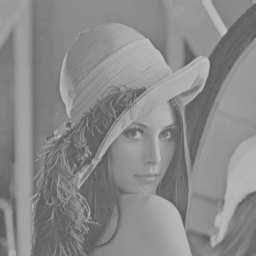
\includegraphics[width=\linewidth]{lena.jpg}
    \caption{Imagem com baixo contraste}
  \end{subfigure}\hfill
  \begin{subfigure}[b]{0.58\linewidth}
    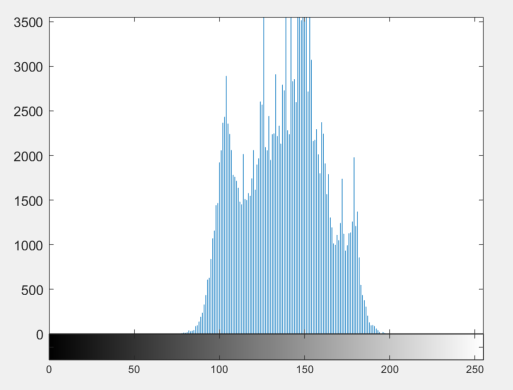
\includegraphics[width=\linewidth]{hist_ckt.png}
    \caption{Histograma concentrado (\textasciitilde{}100--200)}
  \end{subfigure}
\end{figure}

\begin{resposta}

\textbf{Op\c{c}\~ao 1 --- Equaliza\c{c}\~ao de Histograma}

Redistribui os n\'iveis de cinza de forma a maximizar o uso de toda a
faixa $[0, 255]$. A fun\c{c}\~ao de transforma\c{c}\~ao \'e a CDF
normalizada:
\[
  s_k = (L-1)\sum_{j=0}^{k} p_r(r_j)
\]
\textbf{Justificativa:} o histograma da imagem est\'a fortemente
concentrado entre 100 e 200 (estreita gama din\^amica). A equaliza\c{c}\~ao
espalha esses valores por toda a escala, aumentando o contraste global
automaticamente e sem ajuste manual.

\medskip
\textbf{Op\c{c}\~ao 2 --- Alongamento de Contraste
(\textit{Contrast Stretching})}

Aplica uma transforma\c{c}\~ao linear que mapeia o intervalo real
$[r_{\min}, r_{\max}]$ para $[0, 255]$:
\[
  s = \frac{r - r_{\min}}{r_{\max} - r_{\min}} \times 255
\]
\textbf{Justificativa:} como a imagem usa apenas a faixa $\approx
[100, 200]$ dos 256 n\'iveis poss\'iveis, o alongamento linear
redistribui essa faixa para ocupar $[0, 255]$ integralmente,
dobrando efetivamente o contraste sem distorcer a rela\c{c}\~ao relativa
entre as intensidades.

\end{resposta}

%% ================================================================
%% Questão 8 -- Equalização de histograma (4 bits)
%% ================================================================
\begin{questao}[title=Quest\~ao 8 -- Equaliza\c{c}\~ao de Histograma (4\,bits\, $n{=}360$)]
\end{questao}

\begin{resposta}

Imagem de 4\,bits: $L = 16$ n\'iveis ($r_k = 0, 1, \ldots, 15$).
F\'ormula: $s_k = \mathrm{round}\!\left(\dfrac{L-1}{n}\,\mathrm{CDF}(k)\right)$

\begin{center}
\small
\setlength{\tabcolsep}{5pt}
\begin{tabular}{crrccr}
  \toprule
  $r_k$ & $n(r_k)$ & $\text{CDF}$ & $p(r_k)=n/360$ & $s_k$ & $n(s_k)$ \\
  \midrule
  0  & 15  & 15  & 0,0417 & 1  & 15 \\
  1  &  0  & 15  & 0      & 1  & -- \\
  2  &  0  & 15  & 0      & 1  & -- \\
  3  &  0  & 15  & 0      & 1  & -- \\
  4  &  0  & 15  & 0      & 1  & -- \\
  5  &  0  & 15  & 0      & 1  & -- \\
  6  &  0  & 15  & 0      & 1  & -- \\
  7  &  0  & 15  & 0      & 1  & -- \\
  8  &  0  & 15  & 0      & 1  & -- \\
  9  & 70  & 85  & 0,1944 & 4  & 70 \\
  10 & 110 & 195 & 0,3056 & 8  & 110 \\
  11 &  45 & 240 & 0,1250 & 10 &  45 \\
  12 &  80 & 320 & 0,2222 & 13 &  80 \\
  13 &  40 & 360 & 0,1111 & 15 &  40 \\
  14 &   0 & 360 & 0      & 15 & -- \\
  15 &   0 & 360 & 0      & 15 & -- \\
  \midrule
  \textbf{Total} & \textbf{360} & & & & \textbf{360} \\
  \bottomrule
\end{tabular}
\end{center}

\medskip
\textbf{Imagem equalizada --- distribui\c{c}\~ao resultante:}

\begin{center}
\small
\begin{tabular}{ccc}
  \toprule
  $s_k$ & $n(s_k)$ & $p(s_k)$ \\
  \midrule
   1 &  15 & 0,042 \\
   4 &  70 & 0,194 \\
   8 & 110 & 0,306 \\
  10 &  45 & 0,125 \\
  13 &  80 & 0,222 \\
  15 &  40 & 0,111 \\
  \bottomrule
\end{tabular}
\end{center}

Os n\'iveis originais concentrados em $[9,13]$ foram mapeados para
$\{1, 4, 8, 10, 13, 15\}$, espalhando-se ao longo de toda a escala
de 4\,bits e aumentando o contraste da imagem.

\end{resposta}

\end{document}
